
\documentclass[10pt,journal,compsoc]{IEEEtran}

\usepackage[utf8]{inputenc}
\usepackage[T1]{fontenc}
\usepackage{amsmath,amssymb,mathtools}
\usepackage{amsthm}
\usepackage{graphicx}
\usepackage{booktabs}
\usepackage{multirow}
\usepackage{tabularx}
\usepackage{siunitx}
\usepackage{xcolor}
\usepackage{microtype}
\usepackage[colorlinks=true,linkcolor=blue,citecolor=blue,urlcolor=blue]{hyperref}
\usepackage{cleveref}
\usepackage{float}
\usepackage{algorithm}
\usepackage{algorithmic}
\newtheorem{proposition}{Proposition}
\newtheorem{remark}{Remark}
\usepackage[font=small,labelfont=bf,skip=3pt]{caption}
\usepackage{enumitem}
\setlist{nosep,leftmargin=1.2em}

\graphicspath{{figures/}}
\newcommand{\todo}[1]{\textcolor{red}{[TODO: #1]}}
\newcommand{\mgwo}{mGWO}
\newcommand{\mgwoa}{mGWO-a}
\newcommand{\acor}{ACO$_\mathbb{R}$}
\newcommand{\rehap}{REHAP}
\newcommand{\figw}{0.48\columnwidth}

\title{Pitfalls and Benchmarking of Metaheuristic-Tuned Nonlinear Controllers in Robotic Systems: Equal-Budget Validation, Digital Limits, and Generalization}
\author{J.~E.~Cervantes-Reyes,
        Ma.~de~los~Angeles~Alamilla~Daniel,
        and~Angel~Ricardo~Licona~Rodr{\'\i}guez%
\thanks{All authors are with the Universidad Polit\'ecnica de Pachuca, Zempoala, Hidalgo, M\'exico (e-mails: cervantesreyesjesusedg16@gmail.com, alamillameca@upp.edu.mx, arliconar@upp.edu.mx).}}

\begin{document}
\maketitle

\begin{abstract}
Metaheuristics are widely used to tune nonlinear controllers, but studies typically optimize and validate on the same nominal plant, compare methods under unequal budgets, and never test the tuned gains on plants unseen during optimization. We propose a validation protocol for \rehap{}, a two-degree-of-freedom lower-limb rehabilitation robot with a backstepping controller, that trains each independent run on a different perturbed plant and validates on twenty unseen plants under two disturbance patterns. In 30 paired runs with an equal budget of 2000 evaluations, a modified Grey Wolf Optimizer with four escape/intensification mechanisms (\mgwo{}), the canonical GWO, PSO and \acor{} reach statistically indistinguishable validation costs (Friedman $p=0.65$, all Holm-adjusted pairwise $p\ge0.79$); only PSO needs significantly more evaluations to reach its plateau ($p=0.0014$). Activation counters show that one \mgwo{} mechanism never fires and that its exploration schedule never reaches zero within budget; a schedule-corrected variant, \mgwoa{}, recovers most of the lost precision on two benchmark functions (Ackley median $0.108\to0.0094$) but has no effect on controller tuning, and \mgwo{} never outperforms canonical GWO on \rehap{}. We hypothesize that in low-dimensional tuning problems, correct specification of algorithm parameters matters more than the number of escape mechanisms; the evidence is circumstantial and only partly tested.
\end{abstract}

\noindent\textbf{\textit{Keywords}}---rehabilitation robotics, backstepping, controller tuning, robust tuning, grey wolf optimizer, PSO, ACO$_\mathbb{R}$, statistical comparison.

\section{Introduction}
Lower-limb rehabilitation robots must follow prescribed trajectories with small errors. Model-based nonlinear controllers such as backstepping \cite{krstic1995,khalil2002} exploit the Euler--Lagrange structure of the manipulator \cite{spong2006}, and recent designs pair them with disturbance estimation because model uncertainty degrades tracking \cite{peng2022,ren2025}. Performance depends on a few gains whose manual tuning is slow and hard to reproduce. Metaheuristics are a common answer \cite{azeez2023,dai2023}, with GWO \cite{mirjalili2014}, PSO \cite{kennedy1995,shi1998,clerc2002} and \acor{} \cite{socha2008,dorigo1997} as representative families and many GWO variants adding hybrid initialization, mutation, restarts and local search \cite{crepinsek2013,neri2012,blum2003}.

Two practices hamper controller-tuning comparisons: evaluating the optimizer on the same nominal model used to design the controller, and unequal budgets across methods \cite{sorensen2015,camacho2023,kononova2014,kudela2022}. The question that matters to the control engineer, whether the gains work on plants that differ from the model, is seldom answered.

\paragraph{Contributions.}
\begin{enumerate}
\item A validation protocol training on a different perturbed plant per run and validating on 20 unseen plants under two pulse patterns (Sec.~\ref{sec:cost}).
\item Evidence that nominal tuning is uninformative and fragile (Sec.~\ref{sec:results}A--B).
\item An equal-budget, paired, Holm-corrected comparison of \mgwo{}, \mgwoa{}, GWO, PSO and \acor{} over 30 runs (Sec.~\ref{sec:final}).
\item A case study of escape mechanisms: ablation, activation counters and a schedule/budget mismatch tested with a corrected variant (Sec.~\ref{sec:scen}--\ref{sec:hyp}).
\end{enumerate}
The project's original hypothesis, that \mgwo{}'s four mechanisms make it outperform the other optimizers, is \emph{not} supported; we analyze why and formulate a working hypothesis H$^\ast$: in low-dimensional tuning problems, correct specification of algorithm parameters (a schedule consistent with the iterations actually performed, thresholds consistent with the budget) matters more than adding escape mechanisms.

\section{Related Work}
Backstepping is a recursive Lyapunov design for strict-feedback systems \cite{krstic1995,khalil2002}; for a fully actuated manipulator it yields an inverse-dynamics law with a filtered error (Sec.~\ref{sec:control}). GWO \cite{mirjalili2014}, PSO \cite{kennedy1995,shi1998,clerc2002} and \acor{} \cite{socha2008,dorigo1997} balance exploration and exploitation \cite{crepinsek2013} through, respectively, a linearly decaying parameter, inertia and stochastic acceleration, and a sampling distribution built on an elite archive; escape mechanisms such as mutation, restarts and local search (the latter defining memetic search \cite{neri2012,blum2003}) trade evaluations for robustness against stagnation. Both GWO and PSO have been used to tune manipulator controllers \cite{azeez2023,dai2023}.

The metaheuristics literature has questioned novelty claims built on metaphors \cite{sorensen2015,camacho2023} and benchmarks whose optimum sits at the search-space center, which favors methods with a structural bias \cite{kononova2014,kudela2022}; bound-handling choices can also dominate PSO's behavior \cite{helwig2013}. We mitigate the first issue by shifting the optimum of our benchmark functions \cite{suganthan2005,torn1989,ackley1987} away from the origin (Sec.~\ref{sec:scen}) and document the second for PSO (Sec.~\ref{sec:opt}).

Nonparametric tests over independent runs, with the Holm correction \cite{holm1979} for multiple comparisons and the $A_{12}$ effect size \cite{vargha2000}, are the recommended protocol for comparing stochastic optimizers \cite{derrac2011}; the no-free-lunch theorem \cite{wolpert1997} cautions against expecting one method to dominate across problems. Risk-aware objectives such as the conditional value-at-risk \cite{rockafellar2000} are a natural, unused-here alternative to mean-based costs when performance is uncertainty-dependent (Sec.~\ref{sec:disc}). Automatic configuration tools such as \textsc{irace} \cite{lopez2016} are relevant to testing H$^\ast$ (Sec.~\ref{sec:hyp}).

Recent GWO-tuned nonlinear controllers for lower-limb rehabilitation exoskeletons \cite{faraj2023,zheng2026} and GWO-based sliding-mode control for general manipulators \cite{rezoug2022} report gains tuned and validated on the same nominal or fixed-uncertainty plant, with a single optimizer and no equal-budget comparison against alternatives. A scenario-based robust-tuning study on a cart-inverted pendulum \cite{zorlu2026} does train and validate on separate uncertainty scenarios, closer to our protocol, but for a single PID/fractional-order-PID family rather than a multi-optimizer, equal-budget, nonparametric comparison. Table~\ref{tab:sota} makes this gap explicit for the rehabilitation-robotics and manipulator-tuning literature closest to \rehap{}.

\begin{table*}[t]
\centering\footnotesize
\caption{Metaheuristic-tuned nonlinear controllers for manipulators/exoskeletons: validation and comparison practice closest to this work.}
\label{tab:sota}
\begin{tabularx}{\linewidth}{@{}l X X X X@{}}
\toprule
Study & Application & Optimizer(s) & Train/validate on different plants & Equal-budget, multi-optimizer stats\\
\midrule
\cite{azeez2023} & 3-link flexible-joint manipulator & GA-tuned SMC & No (nominal only) & No (single optimizer)\\
\cite{dai2023} & Underwater vehicle-manipulator & GWO & No (nominal only) & No (single optimizer)\\
\cite{faraj2023} & Lower-limb rehab.\ exoskeleton & GWO & No (nominal only) & No (single optimizer)\\
\cite{zheng2026} & Lower-limb rehab.\ exoskeleton & GWO + fuzzy SMC & No (nominal only) & No (single optimizer)\\
\cite{rezoug2022} & Robotic manipulator & Extended GWO & No (nominal only) & No (single optimizer)\\
\cite{zorlu2026} & Cart-inverted pendulum & (FO)PID, scenario-tuned & Yes (uncertainty scenarios) & No (single optimizer family)\\
This work & \rehap{} lower-limb rehab.\ robot & \mgwo{}, GWO, PSO, \acor{} & Yes (20 unseen perturbed plants) & Yes (paired, equal NFE, Friedman/Holm/$A_{12}$)\\
\bottomrule
\end{tabularx}
\end{table*}

\section{System and Controller}\label{sec:model}

\subsection{Euler--Lagrange model}
\rehap{} is an academic test bench (no patient--robot interaction, no clinical validation; see \cite{cervantes2025tesis,cervantes2025congreso}) with two revolute joints $q=[q_1,q_2]^\top$ driven by DC motors with gear ratio $r_i=1$. The Euler--Lagrange model with reflected motor inertia is
\begin{equation}
(M(q)+J_m)\ddot q + C(q,\dot q)\dot q + G(q) + F\dot q = \tau,
\label{eq:dyn}
\end{equation}
with $F=\mathrm{diag}(f_{v1},f_{v2})$, $J_m=\mathrm{diag}(J_{m1},J_{m2})$, and mass-matrix entries $M_{11}=m_1l_{c1}^2+m_2(l_1^2+l_{c2}^2+2l_1l_{c2}\cos q_2)+I_1+I_2$, $M_{12}=M_{21}=m_2(l_{c2}^2+l_1l_{c2}\cos q_2)+I_2$, $M_{22}=m_2l_{c2}^2+I_2$. With $h=m_2l_1l_{c2}\sin q_2$, the Coriolis matrix is
\begin{equation}
C=\begin{bmatrix}-h\dot q_2 & -h(\dot q_1+\dot q_2)\\ h\dot q_1 & 0\end{bmatrix},
\label{eq:coriolis}
\end{equation}
and gravity is
\begin{equation}
G=\begin{bmatrix}(m_1l_{c1}+m_2l_1)g\cos q_1+m_2gl_{c2}\cos(q_1+q_2)\\ m_2gl_{c2}\cos(q_1+q_2)\end{bmatrix}.
\label{eq:gravity}
\end{equation}
For the parameters of Table~\ref{tab:params}, $\det M(q)\ge2.4\times10^{-3}$ over $q_2\in[-\pi,\pi]$ (numerical scan), so $M$ is symmetric positive definite, and $\dot M-2C$ is skew-symmetric as expected for Euler--Lagrange manipulators \cite{spong2006}.

Armature inductance is neglected (no inductance parameter in the model), so the electrical subsystem is algebraic and the torque delivered for armature voltage $v_i$ is
\begin{equation}
\tau_i=\frac{K_a}{R_a}v_i-\frac{K_aK_b}{R_a}\dot q_i,\qquad |v_i|\le v_{\max}=24~\mathrm{V},
\label{eq:motor}
\end{equation}
the physical bottleneck of the actuator ($\tau_{\max}=40$~N\,m is a nominal link limit, not the effective one).

\begin{table*}[t]
\centering\small
\caption{Nominal parameters of \rehap{} (SI units, from the simulation code).}
\label{tab:params}
\begin{tabular}{llllll}
\toprule
$m_1,m_2$ & 7, 1 kg & $l_1$ & 0.50 m & $l_{c1},l_{c2}$ & 0.186, 0.10 m\\
$I_1,I_2$ & $10^{-5}$, $4{\times}10^{-5}$ kg\,m$^2$ & $f_{v1},f_{v2}$ & 0.05 & $J_{m1},J_{m2}$ & 0.062 kg\,m$^2$\\
$K_a=K_b$ & 1.6206 & $R_a$ & 1.8 $\Omega$ & $v_{\max},\tau_{\max}$ & 24 V, 40 N\,m\\
\bottomrule
\end{tabular}
\end{table*}

The reference is a quintic over $T=10$~s from $q_1=-\pi/2$ to $\pi/4$ and $q_2=0$ to $\pi/4$~rad, zero velocity/acceleration at both ends, zero initial error. The loop is integrated with RK4 at $T_s=0.01$~s under zero-order-hold control (100~Hz); sampled-data implementations bound the gains that keep the loop stable \cite{franklin1998} (Sec.~\ref{sec:chatter}).

\subsection{Backstepping controller}\label{sec:control}
With $e=q-q_d$, $K_1=\mathrm{diag}(k_{11},k_{12})$, $K_2=\mathrm{diag}(k_{21},k_{22})$, virtual control $\alpha=\dot q_d-K_1e$ and second-step error $z=\dot q-\alpha=\dot e+K_1e$, the commanded torque is
\begin{equation}
\tau^c=M(q)(\ddot q_d-K_1\dot e-K_2z)+C\dot q+G+F\dot q,
\label{eq:bs_tau}
\end{equation}
and the voltages follow by inverting~\eqref{eq:motor}, adding $J_m\ddot q_r$ ($\ddot q_r=\ddot q_d-K_1\dot e$) to compensate the reflected inertia. The controller uses nominal parameters. For the nominal plant without saturation the error dynamics are
\begin{equation}
\dot z=-\Lambda(q)K_2z,\qquad \dot e=-K_1e+z,\qquad \Lambda=(M+J_m)^{-1}M.
\label{eq:errdyn}
\end{equation}
$\Lambda$ is similar to a symmetric positive definite matrix, so its eigenvalues lie in $(0,1)$; along the reference they range from $0.061$ to $0.908$ (numerical scan), so the slow direction of $z$ decays at only about 6\% of the rate suggested by $K_2$ -- a partial explanation for why optimizers push $k_{22}$ to large values.

\begin{proposition}[Nominal exponential stability, sufficient condition]\label{prop:stability}
For the nominal, continuous-time, unsaturated loop~\eqref{eq:errdyn}, define, for each $q$ along the reference trajectory, $\lambda_2(q):=\lambda_{\min}\bigl(\tfrac12(\Lambda(q)K_2+K_2\Lambda(q)^\top)\bigr)$, the smallest eigenvalue of the symmetric part of $\Lambda(q)K_2$. If $\lambda_{\min}(K_1)>\tfrac12$ and $\inf_q\lambda_2(q)>\tfrac12$ along the reference, the origin $(e,z)=0$ of~\eqref{eq:errdyn} is exponentially stable.
\end{proposition}
\begin{proof}
Let $V=\tfrac12\|e\|^2+\tfrac12\|z\|^2$. Along~\eqref{eq:errdyn}, $\dot V=e^\top\dot e+z^\top\dot z=-e^\top K_1e+e^\top z-z^\top\Lambda K_2z$. Every quadratic form sees only the symmetric part of its matrix, so $z^\top\Lambda K_2z\ge\lambda_2(q)\|z\|^2$ by definition; together with $e^\top z\le\tfrac12\|e\|^2+\tfrac12\|z\|^2$ (Young's inequality),
\[
\dot V\le-\bigl(\lambda_{\min}(K_1)-\tfrac12\bigr)\|e\|^2-\bigl(\lambda_2(q)-\tfrac12\bigr)\|z\|^2\le-2cV,
\]
with $c=\min\{\lambda_{\min}(K_1)-\tfrac12,\ \inf_q\lambda_2(q)-\tfrac12\}>0$ under the stated condition, so $V(t)\le V(0)e^{-2ct}$.
\end{proof}
\begin{remark}
Because $\lambda_{\min}(K_2)\gtrsim\mathcal O(10)$ for every gain set reported here (Table~\ref{tab:final}) while $\lambda_{\min}(\Lambda)\ge0.061$ (above), the condition is easily met component-wise for those gains, but $\Lambda K_2$ is not symmetric, so this is not a proof that $\lambda_2(q)>\tfrac12$ for the reported gains -- only a plausibility argument; $\lambda_2(q)$ was not evaluated directly. Near the lower search bound $lb=1$ the condition can fail outright. Proposition~\ref{prop:stability} is a sufficient condition for the nominal, continuous, unsaturated case only; it does not cover the sampled-data, saturated, or perturbed-plant loop, which is instead assessed numerically (Sec.~\ref{sec:chatter}).
\end{remark}

The tuning variable is $\theta=[k_{11},k_{12},k_{21},k_{22}]^\top$.

\section{Cost, Uncertainty and Protocol}\label{sec:cost}

\subsection{Tracking cost}
For gains $\theta$ the loop is simulated for $T_{sim}=10$~s and
\begin{equation}
\begin{aligned}
J(\theta)={}&\mathrm{RMS}_1+\mathrm{RMS}_2\\
&+\lambda_\tau\overline{\textstyle\sum_i\max(0,|\tau_i^c|-\tau_{\max})^2}+\lambda_{sat}f_{sat},
\end{aligned}
\label{eq:cost}
\end{equation}
where $\mathrm{RMS}_i$ is the true-position tracking error of joint $i$, $\tau^c$ is the torque commanded by~\eqref{eq:bs_tau} before voltage saturation (a proxy of gain aggressiveness, since voltage rather than torque limits the actuator), the overbar is the time average, $f_{sat}$ the fraction of steps with $|v_i|>0.99v_{\max}$, $\lambda_\tau=1$, $\lambda_{sat}=10$ (set after a smoke test, effect not studied). Divergent simulations receive $10^6$.

\subsection{Parametric uncertainty and neuromuscular disturbance pulses}
The plant parameters $\vartheta_k\in\{m_1,m_2,l_{c1},l_{c2},I_1,I_2,f_{v1},f_{v2}\}$ are replaced by
\begin{equation}
\tilde\vartheta_k=\vartheta_k(1+\rho u_k),\qquad u_k\sim\mathcal U(-1,1),\quad \rho=0.15,
\label{eq:uncertainty}
\end{equation}
which represents inter-subject morphological variations (e.g., limb mass and inertia differences in physical therapy), while the controller keeps the nominal model. In rehabilitation robotics, involuntary muscle contractions such as spasticity, tremors, or clonus introduce abrupt joint position perturbations. To reflect these effects during trajectory tracking, a pulse train is added to the measured position,
\begin{equation}
\begin{aligned}
q^m(t)&=q(t)+p(t),\\
p(t)&=\begin{cases}A & t\ge t_0,\ (t-t_0)\bmod P<w\\0&\text{otherwise},\end{cases}
\end{aligned}
\label{eq:pulse}
\end{equation}
with $A=0.01$~rad, $P=2$~s, $w=0.05$~s, $t_0=1$~s (modeling choices; validation also uses an alternative, more aggressive spastic pattern: $A=0.02$~rad, $P=2.5$~s, $w=0.1$~s, $t_0=0.5$~s). Each plant is deterministic given its seed.

\subsection{Optimization problem}\label{sec:probform}
Three settings are used: (A) nominal plant without pulses; (B) one perturbed plant with pulses; (C) the mean of $J$ over five fixed perturbed plants,
\begin{equation}
\bar J(\theta)=\tfrac15\textstyle\sum_{s=1001}^{1005}J(\theta;\mathrm{plant}_s).
\label{eq:barJ}
\end{equation}
The problem is
\begin{equation}
\theta^\star=\arg\min_{\theta\in[lb,ub]}J(\theta),\qquad lb=[1,1,1,1],
\label{eq:optprob}
\end{equation}
with $ub=[1000]^4$ in exploratory experiments and $ub=[1000,1000,1000,600]$ in the final protocol (justified in Sec.~\ref{sec:chatter}). $J$ has no closed-form gradient, is non-smooth (saturation and torque-penalty kinks) and is shaped by discretization artifacts near the digital stability boundary, so we use derivative-free metaheuristics requiring only point-wise evaluations, budgeted in cost evaluations (NFE). In the final protocol, run $k$ trains on a plant with seed $3000+k$, shared by all algorithms (paired design); validation uses twenty plants (seeds 2001--2020) never seen by any optimizer.

\section{Optimization Algorithms}\label{sec:opt}
All optimizers minimize $J$ over the box with the same NFE budget; every evaluation is counted and each run seeds the generator. Table~\ref{tab:hyper} lists the hyperparameters, identical across all experiments.

\paragraph{GWO \cite{mirjalili2014}.} Guides $N$ agents with the three best, $X_\alpha,X_\beta,X_\delta$: $A_\ell=2ar_1-a$, $C_\ell=2r_2$, $X_\ell'=X_\ell-A_\ell\circ|C_\ell\circ X_\ell-X_i|$, $r_1,r_2\sim\mathcal U(0,1)^D$, and $X_i\leftarrow\mathrm{clip}((X_\alpha'+X_\beta'+X_\delta')/3)$, with $a=2(1-t/T_{\max})$, $T_{\max}=\max\{1,\lfloor(NFE_{\max}-N)/N\rfloor\}$. Canonical GWO is not elitist, so we return the best solution seen in the whole run.

\paragraph{\mgwo{}.} Keeps the GWO update and adds: (1) \emph{hybrid initialization}, $n_s$ agents from informed seeds (manual tuning $[5,5,4,4]$ plus four variations); (2) \emph{stagnation mutation}, a counter $c$ resets when the leader improves by $\ge\epsilon$ and grows otherwise, and at $c\ge c_{mut}$ the $n_{mut}$ worst agents mutate; (3) \emph{stagnation recovery} (priority over mutation), a fraction $\phi$ of worst agents re-initializes at $c\ge c_{res}$; (4) \emph{elitist local search}, $n_{loc}$ candidates around $X_\alpha$ replace it only if improved. Mechanisms 2--4 spend extra evaluations, so \mgwo{} completes fewer iterations than GWO in the same budget while $a$ still follows $t/T_{\max}$ (Sec.~\ref{sec:mech}). \mgwoa{} differs only in using $NFE/NFE_{\max}$, instead of $t/T_{\max}$, as the progress variable of $a$ and $r_{loc}$. Algorithm~\ref{alg:mgwo} summarizes the loop; mechanisms 2--4 (\emph{italicized}) are the only departure from canonical GWO.

\begin{algorithm}[t]
\caption{\mgwo{} (canonical GWO update in step 6; \emph{italics} mark the four added mechanisms)}
\label{alg:mgwo}
\begin{algorithmic}[1]
\REQUIRE $N$, $NFE_{\max}$, bounds $[lb,ub]$, $n_s,\epsilon,c_{mut},c_{res},\phi,n_{mut},n_{loc},r_0,\gamma$
\STATE \emph{Initialize $n_s$ agents from informed seeds; the remaining $N-n_s$ uniformly in $[lb,ub]$}
\STATE Evaluate all agents; $NFE\gets N$; $t\gets0$; $c\gets0$
\WHILE{$NFE<NFE_{\max}$}
\STATE Rank agents; set leaders $X_\alpha,X_\beta,X_\delta$; $a\gets2(1-t/T_{\max})$
\FOR{each agent $i=1,\dots,N$}
\STATE $X_i\gets\mathrm{clip}\bigl((X_\alpha'+X_\beta'+X_\delta')/3\bigr)$ \COMMENT{GWO update}
\ENDFOR
\STATE Evaluate updated agents; $NFE\gets NFE+N$
\STATE $c\gets0$ if leader cost improved by $\ge\epsilon$, else $c\gets c+1$
\IF{$c\ge c_{res}$}
\STATE \emph{Stagnation recovery: reinitialize worst $\phi N$ agents uniformly; $c\gets0$}
\ELSIF{$c\ge c_{mut}$}
\STATE \emph{Stagnation mutation: perturb worst $n_{mut}$ agents}
\ENDIF
\STATE \emph{Elitist local search: sample $n_{loc}$ points at radius $r_0(1-t/T_{\max})^\gamma$ around $X_\alpha$; replace $X_\alpha$ only if improved}
\STATE $NFE\gets NFE+$ (evaluations spent above); $t\gets t+1$
\ENDWHILE
\RETURN best solution found over the whole run
\end{algorithmic}
\end{algorithm}

\paragraph{PSO \cite{kennedy1995,shi1998}.} $v\leftarrow wv+c_1r_1\circ(p_i-x)+c_2r_2\circ(g-x)$, $x\leftarrow x+v$, $w$ decreasing linearly, $|v|\le\kappa(ub-lb)$, bounds handled by reflection with velocity inversion \cite{clerc2002}; an earlier clipping version changed final costs by up to $55\times$ across three seeds, consistent with \cite{helwig2013}.

\paragraph{\acor{} \cite{socha2008,dorigo1997}.} Keeps an archive of the $k$ best solutions; each of $m$ ants picks solution $l$ with probability $\propto w_l=\frac{1}{qk\sqrt{2\pi}}e^{-(l-1)^2/(2q^2k^2)}$ and samples each coordinate from a Gaussian centered on it, $\sigma_j=\xi\sum_r|s_r^j-s_l^j|/(k-1)$.

\begin{table*}[t]
\centering\footnotesize
\caption{Optimizer hyperparameters (identical in all experiments).}
\label{tab:hyper}
\begin{tabular}{ll}
\toprule
GWO & $N=20$\\
\mgwo{}, \mgwoa{} & $N=20,\ n_s=5,\ \epsilon=10^{-6},\ c_{mut}=2,\ c_{res}=5,\ \phi=0.2,\ n_{mut}=10,\ \lambda_{mut}=0.05,\ n_{loc}=5,\ r_0=0.1,\ \gamma=2$\\
PSO & $N=20,\ c_1=c_2=2,\ w_{\max}=0.9,\ w_{\min}=0.4,\ \kappa=0.2$\\
\acor{} & $k=50,\ m=5,\ q=0.1,\ \xi=0.85$\\
\bottomrule
\end{tabular}
\end{table*}

\section{Experimental Design}\label{sec:design}
Budgets are in NFE. \textbf{Stage I} (single seed): nominal-plant sweep, $NFE_{\max}=N\cdot iter$ ($k+m\cdot iter$ for \acor{}), $iter\in\{20,50,100,200\}$, plus a digital-stability diagnosis. \textbf{Stage II} (single seed): exploratory multi-plant tuning (setting C, same sweep) with validation on 20 unseen plants. \textbf{Stage III}, the \emph{final protocol}: 30 paired runs, $NFE_{\max}=2000$, setting B with a different training plant per run, validation under two pulse patterns, evaluations to stagnation ($NFE_{5\%}$, $NFE_{1\%}$). \textbf{Stage IV}, pre-declared additional scenarios: S1--S2 (perturbed plant, 300/600 evaluations, 10 seeds; hypothesis: informed seeds and local search help under tight budgets); S3--S4 (Rastrigin \cite{torn1989} and Ackley \cite{ackley1987}, $D=4$, box $[-5.12,5.12]^4$, optimum shifted to $[1.3,-2.1,0.7,-0.9]$ to mitigate center bias \cite{suganthan2005}, 2000 evaluations, 30 seeds, informed seeds disabled; hypothesis: mutation and recovery help on multimodal landscapes); S5 (ablation of each mechanism against GWO, 500 evaluations, 10 seeds); \mgwoa{} was added post hoc to S1--S4 to test H$^\ast$. \textbf{Stage V}: validation of tuned gains on a B\'ezier trajectory (Sec.~\ref{sec:disc}).

Stage III uses the Friedman test, paired Wilcoxon signed-rank tests with Holm correction and $A_{12}$ \cite{derrac2011,holm1979,vargha2000}; S1--S4 use the rank-sum test against \mgwo{} at $\alpha=0.05$, uncorrected (exploratory). Stages I--II support description, not inference. Code is MATLAB R2020a; every scenario, seed and figure is script-generated on a laptop (Intel Core i5-12450HX, 7.7~GB); wall-clock times fluctuated up to 80\% for identical work, so NFE is the primary cost measure.

\section{Results}\label{sec:results}

\subsection{Nominal plant is uninformative}
With 100--200 iterations all optimizers reach $J\approx4.24$--$4.34\times10^{-6}$ (differences $\approx1\%$ among population-based methods): the controller contains the exact model, so nearly any large gains give near-perfect tracking and the problem cannot discriminate optimizers.

\subsection{Digital stability limit}\label{sec:chatter}
The nominal optimum has $k_{22}\approx900$. Varying $k_{22}$ and $T_s$ on the GWO gains (Fig.~\ref{fig:chatter}), the joint-2 error shows no oscillation for $k_{22}\le700$ (peak-to-peak $\le3.6\times10^{-8}$~rad); at $k_{22}\approx902$ a 49.6~Hz component appears (Nyquist: 50~Hz) and vanishes when $T_s$ is halved; at $k_{22}=1000$ the response is unstable. This is consistent with a zero-order-hold effect: the digital stability boundary lies between 700 and 1000 for $T_s=0.01$~s, so the nominal optimum sits at its edge. We take $k_{22}\le600$ as a conservative margin for the final protocol.

\begin{figure}[t]
\centering
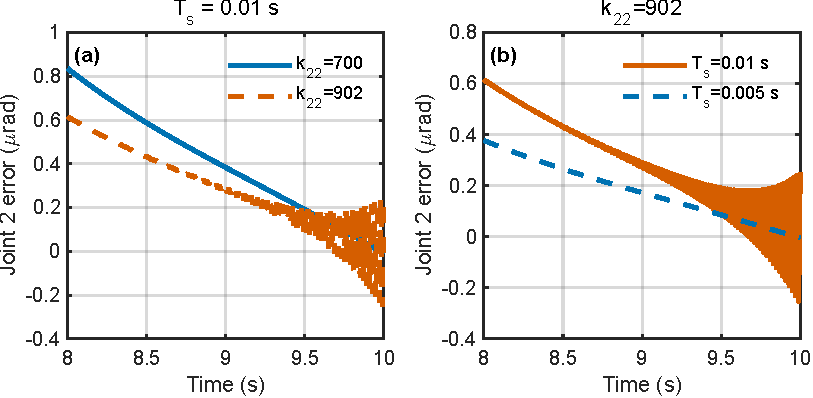
\includegraphics[width=\columnwidth]{articulo/fig_chatter.pdf}
\caption{Joint-2 tracking error in $[8,10]$~s, nominal plant, $\mu$rad (GWO gains, 200 iter.). (a) $T_s=0.01$~s: $k_{22}=700$ is smooth; $k_{22}\approx902$ adds a 49.6~Hz component. (b) $k_{22}\approx902$: halving $T_s$ to 0.005~s removes it.}
\label{fig:chatter}
\end{figure}

\subsection{Fragility under perturbations}\label{sec:fragility}
The 16 nominal gain sets (four optimizers, four budgets), validated on twenty unseen perturbed plants with pulses, reach median cost $1.3\times10^2$--$6.4\times10^3$, worst case $8\times10^4$--$1.1\times10^6$, saturating 7--79\% of the time; gains tuned on five perturbed plants reach $\approx0.026$ (four to five orders of magnitude better) and manual gains $[5,5,4,4]$ obtain $0.60$. Fig.~\ref{fig:loop} shows the mechanism: large nominal gains amplify the pulses and drive the voltage between saturation limits.

\begin{figure}[t]
\centering
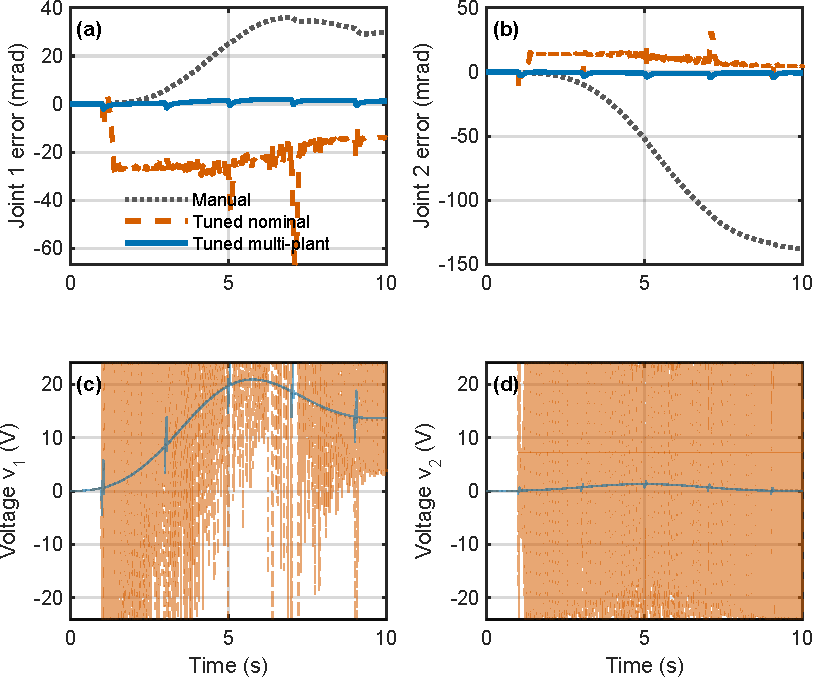
\includegraphics[width=\columnwidth]{articulo/fig_respuesta_lazo.pdf}
\caption{Closed-loop response on one unseen perturbed plant for manual, nominal-tuned and multi-plant-tuned gains (GWO, 200 iter.). (a,b) Tracking errors (mrad); (c,d) armature voltages ($\pm24$~V limits). Nominal gains oscillate between saturation limits (10--30~mrad offset); manual gains avoid saturation but track poorly (up to 140~mrad); multi-plant gains stay within $\approx$10~mrad.}
\label{fig:loop}
\end{figure}

Exploratory multi-plant tuning (single seed, Supplementary~\S S4) already reaches validation medians of 0.0251--0.0260 for $\ge100$ iterations ($\approx24\times$ below manual gains), but the tail persists: 90th percentile $\approx0.7$ and worst case 119--1110, so roughly one plant in ten gives any optimized set a large cost.

\subsection{Final protocol: 30 paired runs}\label{sec:final}
Table~\ref{tab:final}(a) and Fig.~\ref{fig:finalval} summarize the confirmatory experiment. Fig.~\ref{fig:finalval}(a)-(b) show, per algorithm, the distribution over 30 runs of the median validation cost under the training and the alternative pulse pattern; the five boxes overlap almost completely in both panels. Fig.~\ref{fig:finalval}(c) shows the median best training cost against evaluations with its interquartile band, and (d) the evaluations needed to reach 1\% of the final training cost, per run; the four convergence bands in (c) overlap except for PSO's, which trails the others, consistent with the higher per-run counts for PSO visible in (d). Table~\ref{tab:final}(b) adds a B\'ezier-trajectory check on the same tuned gains (Sec.~\ref{sec:disc}).

\begin{table*}[t]
\centering\footnotesize
\caption{(a) Final protocol (30 runs, $NFE_{\max}=2000$): median over runs of the median validation cost on 20 unseen plants under the training pattern ($J_{val}$) and an alternative pattern ($J_{val}^{alt}$), worst validation case, and evaluations to stagnation; IQR is the interquartile range of $J_{val}$ over runs. (b) B\'ezier-trajectory check (nominal plant, no re-optimization) on the manual gains and the median-run gains of \mgwo{} and GWO from panel (a); Sat.\ is the mean \% of saturated steps.}
\label{tab:final}
\begin{tabular}{lrrrrrr}
\multicolumn{7}{l}{\textbf{(a) Final protocol}}\\
\toprule
Algorithm & $J_{val}$ & IQR & $J_{val}^{alt}$ & Worst & $NFE_{5\%}$ & $NFE_{1\%}$\\
\midrule
\mgwo{}  & 0.02616 & 0.0040 & 0.0492 & 509 & 510  & 1398\\
\mgwoa{} & 0.02628 & 0.0030 & 0.0537 & 582 & 403  & 1183\\
GWO      & 0.02619 & 0.0017 & 0.0532 & 628 & 350  & 1220\\
PSO      & 0.02655 & 0.0039 & 0.0545 & 550 & 1320 & 1630\\
\acor{}  & 0.02603 & 0.0018 & 0.0448 & 577 & 645  & 1283\\
\bottomrule
\end{tabular}
\hspace{1em}
\begin{tabular}{lrrrr}
\multicolumn{5}{l}{\textbf{(b) B\'ezier check}}\\
\toprule
Gains & RMSE $q_1$ (rad) & RMSE $q_2$ (rad) & ITSE ($\times10^{-5}$) & Sat.\ (\%)\\
\midrule
Manual $[5,5,4,4]$ & $2.35{\times}10^{-3}$ & $7.38{\times}10^{-3}$ & 4.98 & 0.00\\
\mgwo{} (run 2)    & $1.14{\times}10^{-4}$ & $9.36{\times}10^{-5}$ & 0.011 & 0.00\\
GWO (run 19)       & $1.30{\times}10^{-4}$ & $9.01{\times}10^{-5}$ & 0.015 & 0.00\\
\bottomrule
\end{tabular}
\end{table*}

\paragraph{Quality.} The five algorithms obtain the same validation cost (Fig.~\ref{fig:finalval}a-b): medians 0.02603--0.02655 (2\% spread), Friedman $p=0.65$, all Holm-adjusted pairwise $p\ge0.79$, $A_{12}\in[0.45,0.55]$. With the alternative pattern the omnibus test is not significant either ($p=0.24$). In three of 30 runs all algorithms reach median costs of 0.27--0.78 on shared difficult training plants. \mgwoa{} does not differ from \mgwo{} ($p=1$, $A_{12}=0.46$).

\paragraph{Tails.} No optimizer removes the tail: median-over-runs of the 90th percentile is 0.70--0.72 and of the worst case 509--628 for all algorithms. Training on a different plant per run did not change this, pointing to the cost formulation and plant uncertainty, not the optimizer.

\paragraph{Cost of reaching the plateau.} $NFE_{1\%}$ differs (Friedman $p=0.0014$, Fig.~\ref{fig:finalval}c-d): PSO needs significantly more evaluations than each other algorithm (adjusted $p$ 0.001--0.042), while the other four are indistinguishable (adjusted $p\ge0.44$). All algorithms consume the same NFE, so wall-clock time was essentially equal ($\approx107$~s/run).

\begin{figure}[t]
\centering
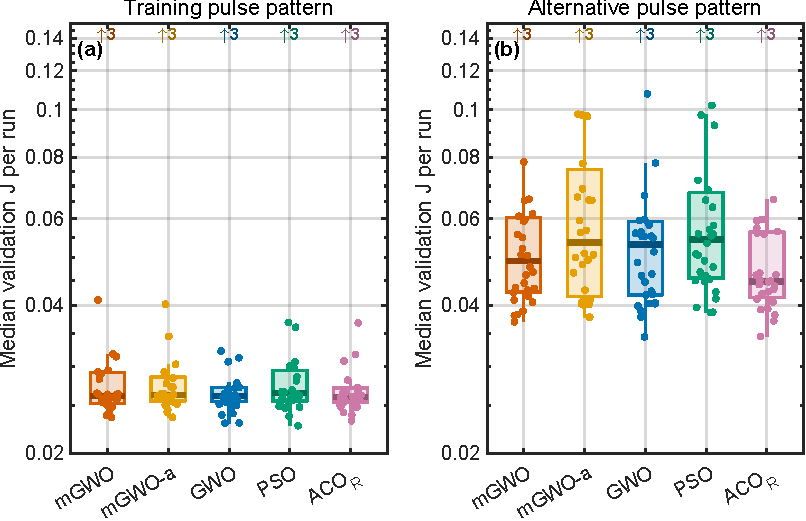
\includegraphics[width=\columnwidth]{articulo/fig_final_validacion.pdf}\\[2pt]
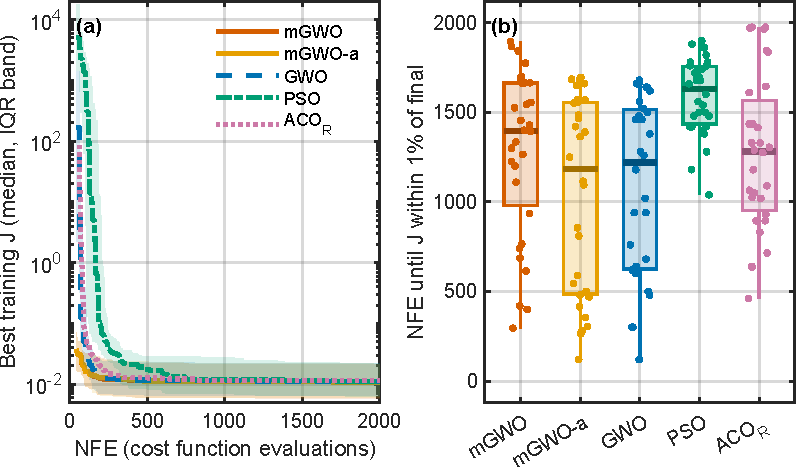
\includegraphics[width=\columnwidth]{articulo/fig_final_convergencia.pdf}
\caption{Final protocol, per-run statistics over 30 runs (log scale). (a) Median validation cost, training pulse pattern; (b) same, alternative pattern. Boxes: quartiles; thick lines: medians; dots: runs. (c) Median best training cost vs.\ evaluations, interquartile band. (d) Evaluations until training cost is within 1\% of its final value, per run. The five algorithms are indistinguishable in (a)-(b); PSO is the only one that visibly lags in (c)-(d).}
\label{fig:finalval}
\end{figure}

\subsection{Additional scenarios}\label{sec:scen}
Table~\ref{tab:scen} summarizes S1--S4; \mgwoa{} rows were added after observing the results.

\begin{table*}[t]
\centering\footnotesize
\caption{Additional scenarios: median final cost (Holm/rank-sum $p$ vs.\ \mgwo{} in parentheses; \textbf{bold}: $p<0.05$).}
\label{tab:scen}
\begin{tabular}{lrrrr}
\toprule
Algorithm & S1 (300 ev.) & S2 (600 ev.) & S3 (Rastrigin) & S4 (Ackley)\\
\midrule
\mgwo{}  & 0.0407 & 0.0402 & 2.98 & 0.108\\
\mgwoa{} & 0.0414 (0.35) & 0.0403 (0.47) & \textbf{2.00 (0.0095)} & \textbf{0.0094 ($3{\times}10^{-11}$)}\\
GWO      & 0.0407 (0.68) & 0.0394 (0.91) & 2.99 (0.60) & \textbf{0.0083 ($8.5{\times}10^{-9}$)}\\
PSO      & \textbf{0.0490 (0.017)} & \textbf{0.0420 (0.031)} & \textbf{1.17 ($1.9{\times}10^{-5}$)} & \textbf{$4.8{\times}10^{-4}$ ($3{\times}10^{-11}$)}\\
\acor{}  & 0.0443 (0.43) & 0.0370 (0.47) & \textbf{5.21 ($1.3{\times}10^{-5}$)} & \textbf{$2.1{\times}10^{-8}$ ($3{\times}10^{-11}$)}\\
\bottomrule
\end{tabular}
\end{table*}

Under tight budgets \mgwo{} equals GWO and \acor{}; its wins against PSO stem from PSO's heavy tail (S1 mean 34.7, driven by one run at 330.6). On benchmarks \mgwo{} equals GWO on Rastrigin, is worse than PSO, and is worse than every algorithm on Ackley, including its own base GWO. \mgwoa{} equals \mgwo{} on \rehap{} but is clearly better on the benchmarks (Rastrigin $2.98\to2.00$; Ackley $0.108\to0.0094$, matching GWO), while PSO/\acor{} remain better on Ackley. In the ablation S5 (500 evaluations, Supplementary~\S S4), no variant differs significantly from full \mgwo{} or GWO (medians 0.0395--0.0407, all $p\ge0.24$); removing local search gives the lowest median, not significantly.

\subsection{Why the mechanisms did not help, and Hypothesis H$^\ast$}\label{sec:mech}\label{sec:hyp}
Activation counters (seed 10) show \mgwo{} completes 19 iterations at 500 evaluations (1 mutation, \emph{no} recovery, 18\% on local search) and 74 iterations at 2000 (13 mutations, no recovery, 18.5\% on local search). Recovery, needing five stagnant iterations, never fired. Because $T_{\max}$ ignores the extra evaluations spent by the mechanisms, \mgwo{} exhausts its budget before $t$ reaches $T_{\max}$: at the end of these runs $a\approx0.42$ and $0.51$ instead of $0$, leaving residual exploration consistent with its poor precision on Ackley.

The evidence for H$^\ast$, circumstantial, is: (i) an escape mechanism was disabled by its threshold relative to the budget; (ii) the schedule of $a$ was inconsistent with the iterations performed, and the algorithm with more mechanisms was worse on Ackley than its own base; (iii) local search consumed $\approx$18\% of evaluations with no measurable benefit; (iv) an implementation detail (PSO bound handling) changed results more than the differences among optimizers; (v) unmodified canonical algorithms matched or exceeded \mgwo{} in most scenarios. \mgwoa{}, which corrects only (ii), supports H$^\ast$ for the schedule component on the benchmarks but not for the controller problem, where all optimizers already share the plateau and the remaining differences lie in the tail. This agrees in direction with work attributing GWO stagnation to the linear schedule of $a$ \cite{li2025} or reliance on three leaders \cite{adegboye2024}; our observation is complementary: budget dependence can silently disable a mechanism or leave $a$ at a wrong value. Thresholds (i), the local-search share (iii) and PSO bound handling (iv) remain untested; automatic configuration \cite{lopez2016} would need to be applied equally to all algorithms.

\section{Discussion}\label{sec:disc}
\paragraph{Interpretation.} No optimizer is best across problems (controller tuning, Rastrigin, Ackley), consistent with \cite{wolpert1997}. A validation of the tuned gains on a B\'ezier trajectory (nominal plant, Table~\ref{tab:final}b) confirms generalization (RMSE falls 20--80$\times$ vs.\ manual gains); on 20 unseen perturbed plants the median gap is kept (12--14$\times$ lower than manual gains) but the tail worsens (worst case 3.6~$\to$~1964 for \mgwo{}, one plant driving most of it via torque saturation), exposing a typical-vs-worst-case trade-off that the median-centered protocol hides (full data in Supplementary~\S S4). This motivates a tail-aware objective such as the conditional value-at-risk \cite{rockafellar2000}.

\paragraph{Limitations.} Stages I--II use a single seed; pulse timing/amplitude are modeling assumptions (mitigated by the alternative pattern); armature inductance is neglected and no formal stability proof is given; cost weights were not studied; findings refer to $D=4$ and do not extrapolate directly to robots with more degrees of freedom; all results are in simulation.

\paragraph{Practical recommendations.} (i)~Never validate gains on the model used to tune them; (ii)~bound gains below the digital stability limit or reduce $T_s$; (iii)~train on perturbed plants, ideally a different one per run, and report tail statistics; (iv)~if quality is equivalent, prefer the optimizer reaching the plateau with fewer evaluations.

\section{Conclusions}\label{sec:concl}
We proposed a validation protocol for robust gain tuning of a backstepping controller on a two-DOF rehabilitation robot and used it for an equal-budget comparison of \mgwo{}, GWO, PSO and \acor{}. Nominal tuning is uninformative and fragile: the optimum sits at the edge of the digital stability region and the gains fail by orders of magnitude under perturbations.

In 30 paired runs the five optimizers delivered the same validation quality (Friedman $p=0.65$); only PSO needed more evaluations to reach the plateau, and none removed the heavy tail. \mgwo{} did not outperform GWO in any scenario and was significantly worse on Ackley; correcting its exploration schedule (\mgwoa{}) recovers benchmark precision but not controller-tuning performance, so the original hypothesis is not supported, while H$^\ast$ is only partly tested. A B\'ezier-trajectory check shows tuned gains improve the median 12--14$\times$ but worsen the worst case.

Future work: (i) complete the H$^\ast$ test with threshold/radius sweeps and equal automatic configuration; (ii) bound $k_{22}$ analytically from the sampled-data condition; (iii) replace the mean by a tail-risk aggregate; (iv) validate on the physical robot.

\paragraph{Supplementary material.} \texttt{supplementary.tex} contains all eliminated figures/tables, full derivations, exploratory-stage results and implementation details.

\begingroup\footnotesize\setlength{\itemsep}{0pt}\setlength{\parsep}{0pt}
\begin{thebibliography}{99}
\bibitem{krstic1995} M.~Krsti\'c, I.~Kanellakopoulos, P.~V. Kokotovi\'c, \emph{Nonlinear and Adaptive Control Design}. Wiley, 1995.
\bibitem{khalil2002} H.~K. Khalil, \emph{Nonlinear Systems}, 3rd ed. Prentice Hall, 2002.
\bibitem{spong2006} M.~W. Spong, S.~Hutchinson, M.~Vidyasagar, \emph{Robot Modeling and Control}. Wiley, 2006.
\bibitem{franklin1998} G.~F. Franklin, J.~D. Powell, M.~L. Workman, \emph{Digital Control of Dynamic Systems}, 3rd ed. Addison-Wesley, 1998.
\bibitem{peng2022} H.~Peng, J.~Zhou, R.~Song, A triple-step controller with linear ADRC for a lower limb rehabilitation robot, \emph{Front.\ Neurorobotics} 16 (2022) 1053360.
\bibitem{ren2025} S.~Ren et al., Command filtered backstepping control with nonlinear disturbance observer for multi-posture lower limb rehabilitation robot, \emph{J.\ Vib.\ Control} (2025). doi:10.1177/10775463251386492.
\bibitem{azeez2023} M.~I. Azeez et al., Optimized sliding mode controller for a flexible-joint three-link manipulator, \emph{Sci.\ Rep.} 13 (2023) 12518.
\bibitem{dai2023} Y.~Dai, D.~Wang, F.~Shen, A robust optimal control by grey wolf optimizer for underwater vehicle-manipulator system, \emph{PLOS ONE} 18 (2023) e0287405.
\bibitem{faraj2023} M.~A. Faraj, B.~Maalej, N.~Derbel, O.~Naifar, Adaptive fractional-order super-twisting sliding mode controller for lower limb rehabilitation exoskeleton in constraint circumstances based on the grey wolf optimization algorithm, \emph{Math.\ Probl.\ Eng.} 2023 (2023) 9641673. doi:10.1155/2023/9641673.
\bibitem{zheng2026} L.~Zheng, M.~Soleimani Amiri, R.~Ramli, N.~H. Mohamed, Adaptive sliding-mode controller with grey wolf optimization and interval type-2 fuzzy logic system for rehabilitation lower-limb exoskeletons, \emph{Biomimetics} 11 (2026) 546. doi:10.3390/biomimetics11080546.
\bibitem{rezoug2022} A.~Rezoug, J.~Iqbal, M.~Tadjine, Extended grey wolf optimization--based adaptive fast nonsingular terminal sliding mode control of a robotic manipulator, \emph{Proc.\ Inst.\ Mech.\ Eng.\ Part I} 236 (2022) 1738--1754. doi:10.1177/09596518221099768.
\bibitem{zorlu2026} H.~Zorlu, M.~T\"urktam, S.~Soylu, Scenario-based robust tuning and generalization analysis of PID and fractional-order PID controllers for a nonlinear cart-inverted pendulum under parametric and disturbance uncertainty, \emph{Appl.\ Sci.} 16 (2026) 8633. doi:10.3390/app16178633.
\bibitem{mirjalili2014} S.~Mirjalili, S.~M. Mirjalili, A.~Lewis, Grey wolf optimizer, \emph{Adv.\ Eng.\ Softw.} 69 (2014) 46--61.
\bibitem{kennedy1995} J.~Kennedy, R.~Eberhart, Particle swarm optimization, in: \emph{Proc.\ IEEE ICNN}, 1995.
\bibitem{shi1998} Y.~Shi, R.~Eberhart, A modified particle swarm optimizer, in: \emph{Proc.\ IEEE ICEC}, 1998, pp.~69--73.
\bibitem{clerc2002} M.~Clerc, J.~Kennedy, The particle swarm---explosion, stability, and convergence, \emph{IEEE Trans.\ Evol.\ Comput.} 6 (1) (2002) 58--73.
\bibitem{helwig2013} S.~Helwig, J.~Branke, S.~Mostaghim, Experimental analysis of bound handling techniques in PSO, \emph{IEEE Trans.\ Evol.\ Comput.} 17 (2) (2013) 259--271.
\bibitem{socha2008} K.~Socha, M.~Dorigo, Ant colony optimization for continuous domains, \emph{Eur.\ J.\ Oper.\ Res.} 185 (2008). doi:10.1016/j.ejor.2006.06.046.
\bibitem{dorigo1997} M.~Dorigo, L.~M. Gambardella, Ant colony system: a cooperative learning approach to the TSP, \emph{IEEE Trans.\ Evol.\ Comput.} 1 (1) (1997) 53--66.
\bibitem{crepinsek2013} M.~\v{C}repin\v{s}ek, S.-H. Liu, M.~Mernik, Exploration and exploitation in evolutionary algorithms: a survey, \emph{ACM Comput.\ Surv.} 45 (3) (2013) 35.
\bibitem{blum2003} C.~Blum, A.~Roli, Metaheuristics in combinatorial optimization: overview and conceptual comparison, \emph{ACM Comput.\ Surv.} 35 (3) (2003) 268--308.
\bibitem{neri2012} F.~Neri, C.~Cotta, Memetic algorithms and memetic computing optimization: a literature review, \emph{Swarm Evol.\ Comput.} 2 (2012) 1--14.
\bibitem{li2025} G.~Li, Y.~Cui, J.~Su, Adaptive mechanism-based grey wolf optimizer for feature selection, \emph{PLOS ONE} 20 (2025) e0318903.
\bibitem{adegboye2024} O.~R. Adegboye et al., Chaotic opposition learning with mirror reflection and worst individual disturbance GWO, \emph{Sci.\ Rep.} 14 (2024) 4660.
\bibitem{sorensen2015} K.~S\"orensen, Metaheuristics---the metaphor exposed, \emph{Int.\ Trans.\ Oper.\ Res.} 22 (1) (2015) 3--18.
\bibitem{camacho2023} C.~L. Camacho-Villal\'on, M.~Dorigo, T.~St\"utzle, Exposing the grey wolf, moth-flame, whale, firefly, bat, and antlion algorithms, \emph{Int.\ Trans.\ Oper.\ Res.} 30 (2023) 2945--2971.
\bibitem{kudela2022} J.~K\r{u}dela, A critical problem in benchmarking and analysis of evolutionary computation methods, \emph{Nat.\ Mach.\ Intell.} (2022). doi:10.1038/s42256-022-00579-0.
\bibitem{kononova2014} A.~V. Kononova et al., Structural bias in population-based algorithms, \emph{Inf.\ Sci.} doi:10.1016/j.ins.2014.11.035.
\bibitem{suganthan2005} P.~N. Suganthan et al., Problem definitions and evaluation criteria for the CEC 2005 special session on real-parameter optimization, KanGAL Report 2005005, Nanyang Technological University, 2005.
\bibitem{torn1989} A.~T\"orn, A.~\v{Z}ilinskas, \emph{Global Optimization}, LNCS 350. Springer, 1989.
\bibitem{ackley1987} D.~H. Ackley, \emph{A Connectionist Machine for Genetic Hillclimbing}. Kluwer, 1987.
\bibitem{cervantes2025tesis} J.~E. Cervantes-Reyes, Sistema de rehabilitaci\'on para extremidades inferiores (REHAP): redise\~no mecatr\'onico, Master's thesis, Universidad Polit\'ecnica de Pachuca, 2025.
\bibitem{cervantes2025congreso} J.~E. Cervantes-Reyes et al., Comparative analysis of nonlinear control strategies for a lower limb rehabilitation system, \emph{Int.\ J.\ Comb.\ Optim.\ Probl.\ Inform.} 16 (3) (2025) 36--45.
\bibitem{wolpert1997} D.~H. Wolpert, W.~G. Macready, No free lunch theorems for optimization, \emph{IEEE Trans.\ Evol.\ Comput.} 1 (1) (1997) 67--82.
\bibitem{lopez2016} M.~L\'opez-Ib\'a\~nez et al., The irace package: iterated racing for automatic algorithm configuration, \emph{Oper.\ Res.\ Perspect.} 3 (2016) 43--58.
\bibitem{rockafellar2000} R.~T. Rockafellar, S.~Uryasev, Optimization of conditional value-at-risk, \emph{J.\ Risk} 3 (2000) 21--41.
\bibitem{derrac2011} J.~Derrac, S.~Garc\'ia, D.~Molina, F.~Herrera, A practical tutorial on nonparametric statistical tests for comparing evolutionary and swarm intelligence algorithms, \emph{Swarm Evol.\ Comput.} 1 (2011). doi:10.1016/j.swevo.2011.02.002.
\bibitem{holm1979} S.~Holm, A simple sequentially rejective multiple test procedure, \emph{Scand.\ J.\ Stat.} 6 (2) (1979) 65--70.
\bibitem{vargha2000} A.~Vargha, H.~D. Delaney, A critique and improvement of the CL common language effect size statistics, \emph{J.\ Educ.\ Behav.\ Stat.} 25 (2) (2000) 101--132.
\end{thebibliography}
\endgroup

\end{document}
